\documentclass{article}

%% Denote paragraphs with vertical space rather than indenting (not critical)
\usepackage{parskip}

%% Support for URL in introductory text (not needed for main example)
\usepackage{url}

%% *** Enable TikZ ***
\usepackage{tikz}


\begin{document}

%% Introductory Text
Example 2.24 from the book\\
\emph{Unlocking LaTeX Graphics: A Concise Guide to Ti$k$Z/PGF and PGFPLOTS}.\\
For more information, visit \url{https://latex-graphics.com}.
\par\bigskip

%% *** START OF EXAMPLE CODE ***
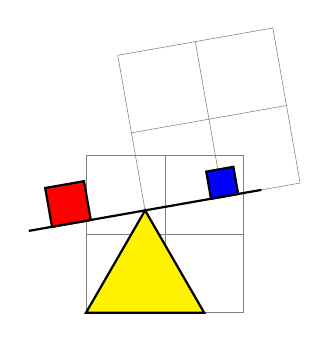
\begin{tikzpicture}[thick]
  \draw[help lines] grid(2,2);
  \draw[scale=0.75,  fill=yellow] (0,0) -- (0:2) -- (60:2) coordinate (tip) -- cycle;
  \begin{scope}[shift=(tip),rotate=10]
    \draw[help lines] grid(2,2);
    \draw (-1.5,0) -- coordinate[pos=0.1] (A)
      coordinate[pos=0.9] (B) (1.5,0);
    \draw[fill=red] (A) rectangle ++(0.5,0.5);
    \draw[fill=blue,scale=0.7] (B) rectangle
      ++(-0.5,0.5);
  \end{scope}
\end{tikzpicture}
%% *** END OF EXAMPLE CODE ***

\end{document}
